\documentclass[state=Report]{mcidoc}
\usepackage{tabularx}
\usepackage{booktabs}                             % Tabellen ohne vertikale Linien (M057)
\usepackage{pgfplots}                             % Diagramme direkt in LaTeX
\pgfplotsset{compat=1.18}

% ---------- Ergänzungen für die MCI-Formalkriterien ----------
\sisetup{locale = UK, uncertainty-mode = separate} % Dezimalpunkt (M030), Unsicherheit mit ± (M031)
\KOMAoptions{listof=totoc}                        % Verzeichnisse erscheinen im Inhaltsverzeichnis
\KOMAoptions{numbers=noendperiod}                 % sonst "Figure 2.1.:" sobald ein Anhang existiert (M018)
\AtBeginEnvironment{table}{\setstretch{1.1}}      % Tabellen kompakter als Fließtext (1.5), einheitlich (M018)
\newenvironment{legendtable}[1]                  % Legende zu Gleichungen (M042), gleicher Zeilenabstand wie Tabellen
  {\par\setstretch{1.1}\noindent\begin{tabular}{#1}}
  {\end{tabular}\par}
\usepackage[autostyle=true]{csquotes}            % englische Anführungszeichen
\usepackage[backend=biber, style=ieee, autocite=superscript]{biblatex}  % IEEE (M080), hochgestellt hinter Satzzeichen (M071): \autocite{...}
\addbibresource{references.bib}
% Hochgestellte Zitate MIT eckigen Klammern, z. B. "...text.^[1]" (M071)
% (Aufbau wie \cite aus numeric-verb, auf dem der IEEE-Stil basiert)
\DeclareCiteCommand{\supercite}[\mkbibsuperscript]
  {\bibopenbracket}
  {\usebibmacro{citeindex}%
   \ifnumgreater{\value{citecount}}{1}
     {\bibopenbracket}
     {}%
   \usebibmacro{cite}}
  {\bibclosebracket\supercitedelim}
  {\bibclosebracket}
\newcounter{romanpage}
% Seitenzahl + Name auch auf Kapitel-Startseiten (Stil "plain"), sonst fehlen sie dort (M010)
\ofoot*{\thepage}
\ifoot*{Mathias Außerlechner, Benedikt Motzet, Urs Müller}  % Fußzeile ohne Studiengang
\KOMAoptions{plainfootsepline=true}

\SetMCI{Language = EN,
    Degree = BSc,
    Title = {Modelling and Control of DC Motor Speed and Position},  % Bezeichnung des Versuchs (Kap. 10.5)
    StudentID = {62200181, 12313575, 52408872},
    % Deckblatt: Namen mit individuellem Studiengang (Kap. 10.5)
    % doppelte Klammern, sonst trennen die Kommas im Studiengang die Schlüsselliste
    % (Fußzeile wird oben mit \ifoot* separat gesetzt)
    Student/Name = {{Mathias Außerlechner (Mechatronics, Design and Innovation)\newline
                    Benedikt Motzet (Mechatronics, Design and Innovation)\newline
                    Urs Müller (Mechatronics, Design and Innovation)}},
    Report/Supervisor/Name = {FH-Prof. Yeongmi Kim, PhD},
    Report/Cohort = {BA-MECH-24-4C},
    Report/Lecture = {Control Engineering \uppercase\expandafter{\romannumeral 2} -- Laboratory},  % Laborübung
    Report/Date = {October 16, 2026},  % Labortermin (Vorgabe Laboranleitung)
    Report/Mode = Lab,                 % "Lab Supervisor" auf dem Deckblatt
    Report/ToC/Primary = unset,        % Verzeichnisse setzen wir unten selbst
    Report/ToC/Figures = unset,
    Report/ToC/Tables  = unset,
}

\begin{document}

% ---------- Vorspann: römische Seitenzahlen (M010) ----------
\pagenumbering{Roman}
\tableofcontents
\clearpage
\setcounter{romanpage}{\value{page}}
\pagenumbering{arabic}

% ---------- Hauptteil: arabische Seitenzahlen ----------
\chapter{Introduction}\label{ch:introduction}

\section{General Description}\label{sec:general}
This report documents the modelling, identification and position control of a
DC motor that drives a pointer via a gearbox with belt drive (Box~1 of the
laboratory test benches). The controlled variable is the angular position of the
pointer, measured on the output shaft by an optical quadrature encoder. The motor
is supplied by a PWM-controlled motor driver, and all signals are processed by a
data acquisition card with MATLAB/Simulink and Simulink Desktop
Real-Time\autocite{laboranleitung}.

\section{Motivation}\label{sec:motivation}
DC motors are widely used electro-mechanical actuators, for example in
automotive applications, medical devices and industrial
automation\autocite{laboranleitung}. An exact positioning of the driven load
requires a closed-loop controller, whose design relies on a sufficiently
accurate model of the plant. Since not all parameters of a real drive train are
known, the model is derived both analytically and from measured data.

\section{Learning Goal}\label{sec:goal}
The aim of the laboratory is to identify an electro-mechanical system from its
measured step response and to design a suitable controller\autocite{laboranleitung}.
The step response is approximated by a second-order lag element, a PID
controller is designed with the Ziegler--Nichols method, and the closed loop is
simulated, implemented on the real test bench and evaluated.

\chapter{Procedure and Method}\label{ch:procedure}

\section{Experimental Setup}\label{sec:setup}
% Versuchsskizze (M086): beschriftete Abbildung des Aufbaus einfügen.
The equipment is listed in Table~\ref{tab:equipment}; the labelled test bench is
shown in Figure~\ref{fig:testbench} in Appendix~\ref{app:schematic}.

\begin{table}[H]
  \centering
  \caption[List of equipment]{List of equipment used for the experiment
   \autocite{laboranleitung}}
  \label{tab:equipment}
  \begin{tabularx}{\textwidth}{l >{\raggedright\arraybackslash}X l}
    \toprule
    Component & Description & Type \\
    \midrule
    Test bench   & gearbox with belt drive, Box~1, $N = \num{97.2}$ & -- \\
    DC motor     & brushed, nominal voltage \qty{12}{\volt}
                 & Faulhaber 3257G012CR\autocite{faulhaber3257} \\
    Motor driver & PWM-controlled motor driver & Cytron MD13S\autocite{cytronMD13S} \\
    Encoder      & quadrature, \num{500} counts per revolution
                 & Broadcom HEDS-5500 A11\autocite{heds5500} \\
    DAQ card     & data acquisition card & NI PCIe-6321\autocite{niXseries} \\
    I/O module   & BNC connector block & NI BNC-2090a \\
    Software     & simulation and real-time control
                 & MATLAB/Simulink R2020b, R2024b \\
    \bottomrule
  \end{tabularx}
\end{table}

\section{Analytical Modelling of the DC Motor}\label{sec:modelling}
% Quelle: eigene Vorbereitung (preperation31final.mlx), Ersatzschaltbild aus [1]
The unloaded DC motor is described by a white-box model based on
Figure~\ref{fig:schematic} in Appendix~\ref{app:schematic}, with the motor
quantities written without the index \enquote{mot}, $U_\mathrm{in}$ as $u$,
$U_\mathrm{emf}$ as $u_\mathrm{emf}$ and the rotation $n_\mathrm{out}$
described by $\omega$. Kirchhoff's voltage law for the armature circuit with the back electromotive
force $u_\mathrm{emf} = k_\mathrm{E}\,\omega$ yields
Equation~\eqref{eq:electrical}, the balance of torques at the rotor yields
Equation~\eqref{eq:mechanical}.
\begin{equation}
  u(t) = R\,i(t) + L\,\frac{\mathrm{d}i(t)}{\mathrm{d}t} + k_\mathrm{E}\,\omega(t)
  \label{eq:electrical}
\end{equation}
\begin{equation}
  J\,\frac{\mathrm{d}\omega(t)}{\mathrm{d}t} = k_\mathrm{M}\,i(t) - b\,\omega(t)
  \label{eq:mechanical}
\end{equation}
% Legende zu den zentralen Gleichungen (M042)
\begin{legendtable}{@{}l@{\quad}l@{\qquad}l@{\quad}l@{}}
  $u$        & armature voltage, in \unit{\volt}
    & $J$            & rotor inertia, in \unit{\kilogram\metre\squared} \\
  $i$        & armature current, in \unit{\ampere}
    & $b$            & viscous friction, in \unit{\newton\metre\second\per\radian} \\
  $\omega$   & angular velocity, in \unit{\radian\per\second}
    & $k_\mathrm{M}$ & torque constant, in \unit{\newton\metre\per\ampere} \\
  $R$        & armature resistance, in \unit{\ohm}
    & $k_\mathrm{E}$ & back-EMF constant, in \unit{\volt\second\per\radian} \\
  $L$        & armature inductance, in \unit{\henry}
    & $t$            & time, in \unit{\second}
\end{legendtable}

\noindent
With $\omega = \mathrm{d}\theta/\mathrm{d}t$ for the angular position $\theta$,
the Laplace transformation with zero initial conditions gives
\begin{equation*}
  U(s) = (R + L s)\, I(s) + k_\mathrm{E}\, s\, \Theta(s), \qquad
  J s^2\, \Theta(s) = k_\mathrm{M}\, I(s) - b\, s\, \Theta(s),
\end{equation*}
where capital letters denote Laplace transforms and $s$ is the Laplace variable.
Solving the mechanical equation for $I(s) = (J s^2 + b s)\,\Theta(s)/k_\mathrm{M}$
and substituting it into the electrical equation yields
\begin{equation*}
  U(s) = \left[ \frac{(R + L s)(J s^2 + b s)}{k_\mathrm{M}} + k_\mathrm{E}\, s \right] \Theta(s)
  = \frac{s \left[ L J s^2 + (R J + L b)\, s + (R b + k_\mathrm{E} k_\mathrm{M}) \right]}
         {k_\mathrm{M}}\, \Theta(s).
\end{equation*}
Hence, the transfer function to the angular position in Equation~\eqref{eq:gp1}
is of third order with an integrator, and with $\Omega(s) = s\,\Theta(s)$ the one
to the angular velocity in Equation~\eqref{eq:gp2} is a PT2 element, which
justifies the PT2 approach in Section~\ref{sec:identification}.
\begin{equation}
  G_\mathrm{p1}(s) = \frac{\Theta(s)}{U(s)}
  = \frac{k_\mathrm{M}}{s \left[ L J s^2 + (R J + L b)\, s + (R b + k_\mathrm{E} k_\mathrm{M}) \right]}
  \label{eq:gp1}
\end{equation}
\begin{equation}
  G_\mathrm{p2}(s) = \frac{\Omega(s)}{U(s)} = s\,G_\mathrm{p1}(s)
  = \frac{k_\mathrm{M}}{L J s^2 + (R J + L b)\, s + (R b + k_\mathrm{E} k_\mathrm{M})}
  \label{eq:gp2}
\end{equation}
With the state variables
$\mathbf{x} = \begin{bmatrix} \theta & \omega & i \end{bmatrix}^\mathrm{T}$,
the input $u$ and the output $\theta$, rearranging Equations~\eqref{eq:electrical}
and~\eqref{eq:mechanical} for the derivatives gives the state-space model
$\dot{\mathbf{x}} = \mathbf{A}\mathbf{x} + \mathbf{b}\,u$,
$\theta = \mathbf{c}^\mathrm{T}\mathbf{x}$ with
\begin{equation*}
  \mathbf{A} =
  \begin{bmatrix}
    0 & 1 & 0 \\
    0 & -b/J & k_\mathrm{M}/J \\
    0 & -k_\mathrm{E}/L & -R/L
  \end{bmatrix}, \qquad
  \mathbf{b} = \begin{bmatrix} 0 \\ 0 \\ 1/L \end{bmatrix}, \qquad
  \mathbf{c}^\mathrm{T} = \begin{bmatrix} 1 & 0 & 0 \end{bmatrix}.
\end{equation*}

\section{System Identification}\label{sec:identification}
% Daten: matlab.mat (resp_12V), Fit: squarefit.m / PT2.m
The step response is recorded for an input step of $u_0 = \qty{12}{\volt}$ at
$t = \qty{0}{\second}$ (sample time \qty{0.1}{\milli\second}).\autocite{laboranleitung}
The rotational speed $n$ of the output shaft in \unit{\per\minute} is converted
into $\omega = 2\pi n / \qty{60}{\second\per\minute}$, which is lower than the
motor speed by the factor $N$. The plant is approximated by an overdamped PT2
element according to Equation~\eqref{eq:pt2} with the static gain $K$ in
\unit{\radian\per\second\per\volt} and the time constants $\tau_1$, $\tau_2$ in
\unit{\second}.
\begin{equation}
  G_\mathrm{PT2}(s) = \frac{\Omega(s)}{U(s)}
  = \frac{K}{(\tau_1 s + 1)(\tau_2 s + 1)}
  \label{eq:pt2}
\end{equation}
$K$, $\tau_1$ and $\tau_2$ are determined by a least-squares fit of the step
response
\begin{equation*}
  \omega(t) = u_0 K \left[ 1 - \frac{\tau_1\,\mathrm{e}^{-t/\tau_1}
  - \tau_2\,\mathrm{e}^{-t/\tau_2}}{\tau_1 - \tau_2} \right]
\end{equation*}
to the measurement with the MATLAB function \texttt{lsqcurvefit}. The preparatory
identification is given in Appendix~\ref{app:prep}. Integrating
the angular velocity gives the plant for the position control in
Equation~\eqref{eq:pt3}\autocite{laboranleitung}.
\begin{equation}
  G_\mathrm{p}(s) = \frac{\Theta(s)}{U(s)} = \frac{1}{s}\,G_\mathrm{PT2}(s)
  = \frac{K}{s\,(\tau_1 s + 1)(\tau_2 s + 1)}
  \label{eq:pt3}
\end{equation}

\section{Controller Design and Implementation}\label{sec:design}
% Ziegler--Nichols Methode 2 (squarefit.m): rlocus -> K_cr, P_cr
A PID controller according to Equation~\eqref{eq:pid} with the proportional
gain $K_\mathrm{P}$ in \unit{\volt\per\radian}, the integral and derivative times
$T_\mathrm{I}$, $T_\mathrm{D}$ in \unit{\second}, $K_\mathrm{I} = K_\mathrm{P}/T_\mathrm{I}$
and $K_\mathrm{D} = K_\mathrm{P}\,T_\mathrm{D}$ is designed with the closed-loop
method of Ziegler and Nichols\autocite{ziegler1942}.
\begin{equation}
  G_\mathrm{c}(s) = K_\mathrm{P} \left( 1 + \frac{1}{T_\mathrm{I}\,s}
  + T_\mathrm{D}\,s \right)
  = K_\mathrm{P} + \frac{K_\mathrm{I}}{s} + K_\mathrm{D}\,s
  \label{eq:pid}
\end{equation}
The critical gain $K_\mathrm{cr}$, at which the closed loop of $G_\mathrm{p}(s)$
with a pure P controller reaches the stability limit, is determined from the
root locus with the MATLAB function \texttt{rlocus}, and the period
$P_\mathrm{cr}$ of the sustained oscillation from the simulated output
signal\autocite{laboranleitung}. The tuning rules $K_\mathrm{P} = 0.6\,K_\mathrm{cr}$,
$T_\mathrm{I} = 0.5\,P_\mathrm{cr}$ and $T_\mathrm{D} = 0.125\,P_\mathrm{cr}$
then give the controller parameters\autocite{ziegler1942}. The closed loop is
simulated in Simulink, with the reference converted from degrees into radians
before the controller and the output converted back\autocite{laboranleitung}.

\label{sec:implementation}
% Einstellungen aus RunPositionController1.slx, Parameter aus Controll_eng_pid_tuning.xlsx
The controller is implemented in Simulink Desktop Real-Time (sample time
\qty{0.1}{\milli\second}) in the parallel form of Equation~\eqref{eq:pid} with a
first-order derivative filter (coefficient \qty{100}{\per\second}), a control
value limit of \qty{\pm 12}{\volt} and clamping anti-windup. For each run, a
\ang{45} reference step is recorded for \qty{1}{\second} while $K_\mathrm{P}$,
$K_\mathrm{I}$ and $K_\mathrm{D}$ are varied; a manual disturbance and a
sinusoidal reference are also tested.

\chapter{Results}\label{ch:results}
% GRUNDSATZ: Nur eigene Ergebnisse und Messungen der Gruppe verwenden
% (Lab_bennimathiasurs: squarefit.m, PT2.m, matlab.mat, Controll_eng_pid_tuning.xlsx).

\section{Identified Transfer Function}\label{sec:res-identification}
% Quelle: squarefit.m (lsqcurvefit mit PT2.m), Ergebnis X in matlab.mat
% Daten: data/step_response_12V.csv (resp_12V, Drehzahl / 9.55 wie in squarefit.m,
%        Modellkurve = PT2(X, t), jede 50. Abtastung)
The least-squares fit yields the parameters
$K = \qty{0.4334}{\radian\per\second\per\volt}$,
$\tau_1 = \qty{0.0076}{\second}$ and $\tau_2 = \qty{0.1030}{\second}$.
Measurement and identified model are compared in
Figure~\ref{fig:identification}. As an example of the conversion of the
measured data, the last recorded sample with $n = \qty{50}{\per\minute}$
corresponds to
\begin{equation*}
  \omega = \frac{2\pi\,n}{\qty{60}{\second\per\minute}}
  = \frac{2\pi \cdot \qty{50}{\per\minute}}{\qty{60}{\second\per\minute}}
  = \qty{5.24}{\radian\per\second}.
\end{equation*}

\begin{figure}[H]
  \centering
  \begin{tikzpicture}
    \begin{axis}[
        width=0.8\textwidth, height=0.36\textwidth,
        xlabel={$t$/\unit{\second}}, ylabel={$\omega$/(\unit{\radian\per\second})},
        xmin=0, xmax=1.5, ymin=0, ymax=6,
        grid=major, grid style={gray!30},
        legend pos=south east, legend cell align=left,
        /pgf/number format/.cd, use period,
      ]
      \addplot[black, dotted, thick]
        table[x=t, y=omega_meas, col sep=comma] {data/step_response_12V.csv};
      \addlegendentry{measurement}
      \addplot[black]
        table[x=t, y=omega_model, col sep=comma] {data/step_response_12V.csv};
      \addlegendentry{identified PT2 model}
    \end{axis}
  \end{tikzpicture}
  \caption[Measured and identified step response]{Measured angular velocity of
    the output shaft (dotted) and step response of the identified PT2 model
    (solid) for an input step of \qty{12}{\volt}}
  \label{fig:identification}
\end{figure}

With Equation~\eqref{eq:pt3}, the plant for the position control is
\begin{equation*}
  G_\mathrm{p}(s) = \frac{\qty{0.4334}{\radian\per\second\per\volt}}
  {s\,(\qty{0.0076}{\second} \cdot s + 1)(\qty{0.1030}{\second} \cdot s + 1)}.
\end{equation*}

\section{Controller Parameters and Simulation}\label{sec:res-simulation}
% Quelle: squarefit.m (kcr = 325 aus root locus, pcr = 0.175701 s, kp, Ti, Td, ki, kd)
From the root locus of $G_\mathrm{p}(s)$, a critical gain of
$K_\mathrm{cr} = \qty{325}{\volt\per\radian}$ and a period of
$P_\mathrm{cr} = \qty{0.1757}{\second}$ are obtained. The tuning rules give
$K_\mathrm{P} = 0.6 \cdot \qty{325}{\volt\per\radian} = \qty{195}{\volt\per\radian}$,
$T_\mathrm{I} = 0.5 \cdot \qty{0.1757}{\second} = \qty{0.0879}{\second}$ and
$T_\mathrm{D} = 0.125 \cdot \qty{0.1757}{\second} = \qty{0.0220}{\second}$, and thus
\begin{equation*}
  K_\mathrm{I} = \frac{K_\mathrm{P}}{T_\mathrm{I}}
  = \frac{\qty{195}{\volt\per\radian}}{\qty{0.0879}{\second}}
  = \qty{2219.7}{\volt\per\radian\per\second}
\end{equation*}
and $K_\mathrm{D} = K_\mathrm{P}\,T_\mathrm{D}
= \qty{195}{\volt\per\radian} \cdot \qty{0.0220}{\second}
= \qty{4.28}{\volt\second\per\radian}$.
The simulated step response of the closed loop with the adjusted integral gain
(see Section~\ref{sec:res-realtime}) is shown in Figure~\ref{fig:simulation}.

% VORLÄUFIG (vor Abgabe durch eigenen Export ersetzen):
% erzeugt von Claude durch unveränderten Lauf von Lab_bennimathiasurs/PID_simulation.slx
% (oberer Kreis mit D2R, Sättigung ±12 V, R2D; Sollwert 20 deg, K_P = 195, K_I = 22.197,
% K_D = 4.2827, N = 100, kein Anti-Windup). Daten: data/simulation_closed_loop.csv (0--1 s,
% Solver-Ausgabe linear auf 0.5 ms interpoliert).
\begin{figure}[H]
  \centering
  \begin{tikzpicture}
    \begin{axis}[
        name=top, width=0.8\textwidth, height=0.3\textwidth,
        ylabel={$\theta$, $r$, $e$/\unit{\degree}},
        xmin=0, xmax=1, ymin=-5, ymax=25, xticklabels={},
        grid=major, grid style={gray!30},
        legend style={at={(0.98,0.5)}, anchor=east}, legend columns=3, legend cell align=left,
        legend style={font=\footnotesize},
        /pgf/number format/.cd, use period,
      ]
      \addplot[black, thick] table[x=t, y=theta, col sep=comma] {data/simulation_closed_loop.csv};
      \addlegendentry{position $\theta$}
      \addplot[black, dotted, thick] table[x=t, y=r, col sep=comma] {data/simulation_closed_loop.csv};
      \addlegendentry{reference $r$}
      \addplot[black, dashed] table[x=t, y=e, col sep=comma] {data/simulation_closed_loop.csv};
      \addlegendentry{error $e$}
    \end{axis}
    \begin{axis}[
        at={(top.below south west)}, anchor=north west, yshift=-0.3em,
        width=0.8\textwidth, height=0.22\textwidth,
        xlabel={$t$/\unit{\second}}, ylabel={$u$/\unit{\volt}},
        xmin=0, xmax=1, ymin=-15, ymax=15,
        grid=major, grid style={gray!30},
        /pgf/number format/.cd, use period,
      ]
      \addplot[black, thick] table[x=t, y=u, col sep=comma] {data/simulation_closed_loop.csv};
    \end{axis}
  \end{tikzpicture}
  \caption[Simulated closed-loop step response]{Simulated closed-loop response
    for a reference step of \ang{20} with
    $K_\mathrm{P} = \qty{195}{\volt\per\radian}$,
    $K_\mathrm{I} = \qty{22.2}{\volt\per\radian\per\second}$,
    $K_\mathrm{D} = \qty{4.28}{\volt\second\per\radian}$ and a control value
    limited to \qty{\pm 12}{\volt}: angular position, reference and control
    error (top) and control value (bottom)}
  \label{fig:simulation}
\end{figure}

\section{Real-Time Control}\label{sec:res-realtime}
% Quelle: Controll_eng_pid_tuning.xlsx (Verstärkungen und Kommentare),
%         matlab.mat (M1--M8, disturbance, sine ... sine5)
Table~\ref{tab:runs} lists the controller gains of all runs with a reference
step of \ang{45} together with the observations noted during the laboratory.
The measured step responses are shown in Figures~\ref{fig:run1}
to~\ref{fig:run8} in Appendix~\ref{app:steps}.

\begin{table}[H]
  \centering
  \caption[Controller gains of the real-time runs]{Controller gains and
    observations of the real-time runs for a reference step of \ang{45}}
  \label{tab:runs}
  \begin{tabular}{
      S[table-format=1.0]
      S[table-format=3.0]
      S[table-format=4.1]
      S[table-format=1.2]
      l
    }
    \toprule
    {Run} & {$K_\mathrm{P}$/(\unit{\volt\per\radian})}
      & {$K_\mathrm{I}$/(\unit{\volt\per\radian\per\second})}
      & {$K_\mathrm{D}$/(\unit{\volt\second\per\radian})} & Observation \\
    \midrule
    1 & 195 &   22.2 & 4.28 & $K_\mathrm{I}$ adjusted \\
    2 & 195 & 2219.7 & 4.28 & calculated (Ziegler--Nichols) \\
    3 &   1 &   22.2 & 4.28 & $K_\mathrm{P}$ reduced \\
    4 &  20 &   22.2 & 4.28 & $K_\mathrm{P}$ reduced \\
    5 & 195 &   22.2 & 8.00 & $K_\mathrm{D}$ increased \\
    6 & 195 &   22.2 & 1.00 & $K_\mathrm{D}$ reduced, overshoot \\
    7 & 300 &   22.2 & 4.28 & $K_\mathrm{P}$ increased \\
    8 & 300 &   22.2 & 6.00 & $K_\mathrm{P}$ and $K_\mathrm{D}$ increased \\
    \bottomrule
  \end{tabular}
\end{table}

With the calculated Ziegler--Nichols parameters (run~2), the position overshoots
the reference before it settles (Figure~\ref{fig:run2}). With $K_\mathrm{I}$
reduced by a factor of 100 (run~1), the reference is reached without visible
overshoot (Figure~\ref{fig:run1}); these parameters are the starting point for
the further variations. With the strongly reduced proportional gains of runs~3
and~4, the position rises slowly, is still moving at the end of the recording and
exceeds the reference. Increasing $K_\mathrm{D}$ (run~5) leads to a response
without overshoot, whereas reducing $K_\mathrm{D}$ (run~6) causes an overshoot.
The step responses with increased $K_\mathrm{P}$ (run~7) and additionally
increased $K_\mathrm{D}$ (run~8) are shown in Figures~\ref{fig:run7}
and~\ref{fig:run8}. In all runs, the recorded control value reaches the
saturation limit of \qty{12}{\volt} directly after the reference step.

With the gains of run~1, a disturbance is applied manually to the pointer
(Figure~\ref{fig:disturbance} in Appendix~\ref{app:data}): the pointer is
deflected by approximately \ang{2} and is returned to the reference by the
controller. For the tracking of a sinusoidal reference
(Table~\ref{tab:sine} and Figures~\ref{fig:sine-track} to~\ref{fig:sine1200} in
Appendix~\ref{app:data}), the response with $K_\mathrm{P} = \qty{195}{\volt\per\radian}$
is observed to be slightly slow. Increasing $K_\mathrm{P}$ to
\qty{300}{\volt\per\radian} halves the control error, and
\qty{600}{\volt\per\radian} reduces it further, while at
\qty{800}{\volt\per\radian} and \qty{1200}{\volt\per\radian} the control value
becomes strongly noisy.

\chapter{Discussion and Interpretation}\label{ch:discussion}
% GRUNDSATZ: Nur Ergebnisse/Messungen der Gruppe interpretieren, keine neuen Berechnungen.
% Analytische Werte: Aufgabe31LAB1.mlx (Datenblattwerte Faulhaber 3257G012CR)

\section{Comparison of Measurement, Model and Simulation}\label{sec:comparison}
The identified PT2 model reproduces the measured step response of the angular
velocity well (Figure~\ref{fig:identification}): both the rise and the
stationary value are matched, and the remaining deviations are mainly caused by
the noise of the measured signal. This noise results from the calculation of the
rotational speed from the position change of the incremental encoder between
two samples\autocite{laboranleitung}, so that the speed is only available in
discrete steps. The overdamped PT2 structure therefore describes the dynamic
behaviour of the drive sufficiently for the controller design, which is
consistent with the analytical model in Equation~\eqref{eq:gp2}. The same
approach was already successful for the preparatory data, where an additional
dead time was required to describe the delayed reaction of the system
(Appendix~\ref{app:prep}).

A comparison with the analytical model shows clear differences. Evaluating
Equation~\eqref{eq:gp2} with the datasheet values of the motor\autocite{faulhaber3257}
yields a static gain of \qty{52.36}{\radian\per\second\per\volt} and time
constants of \qty{4.5}{\milli\second} and \qty{0.18}{\milli\second}. The static
gain refers to the motor shaft, whereas the identified gain refers to the output
shaft; both are therefore only comparable when the transmission ratio $N$ is
taken into account, which brings them into the same order of magnitude. The time
constants, however, differ substantially: the dominant identified time constant
$\tau_2 = \qty{0.1030}{\second}$ is more than an order of magnitude larger than
the analytical one. The main reason is the assumption of an unloaded motor in the
analytical model. The real test bench additionally contains the gearbox, the
belt drive and the pointer, whose inertia and friction slow down the system
considerably. Furthermore, the motor driver and the real friction behaviour are
not part of the analytical model. The analytical model is thus suitable to
justify the model structure, while the parameters for the controller design have
to be identified experimentally.

% TODO: Vergleich Simulation (Figure 3.2) <-> Messung (Runs 1 und 2) ergänzen,
% sobald die Simulationsergebnisse aus PID_simulation.slx vorliegen.

\section{Controller Performance}\label{sec:performance}
The controller designed with the Ziegler--Nichols method stabilises the position
control loop, but the step response with the calculated parameters (run~2)
shows an overshoot (Figure~\ref{fig:run2}). This is expected, since the tuning
rules of Ziegler and Nichols aim at a fast response with a decay ratio of about
one quarter rather than at a response without overshoot\autocite{ziegler1942}. The
Ziegler--Nichols parameters are therefore a starting point that has to be
adjusted on the real system.

The most effective adjustment is the reduction of the integral gain by a factor
of 100 (run~1), after which no overshoot is visible (Figure~\ref{fig:run1}). This
can be explained by the structure of the plant: $G_\mathrm{p}(s)$ already
contains an integrator, so that a constant reference is reached without
remaining control error even without integral action. A large integral gain
mainly accumulates the control error during the rise and thus causes the
overshoot. A small integral gain is nevertheless useful, since it compensates
constant disturbances such as friction torques. This is confirmed by the
disturbance test (Figure~\ref{fig:disturbance}), in which the manually deflected
pointer is returned to the reference.

The variation of the gains shows the expected tendencies. A strongly reduced
proportional gain (runs~3 and~4) leads to a slow response that has not settled
at the end of the recording (Figures~\ref{fig:run3} and~\ref{fig:run4}). Since
the proportional part provides only a small control value in this case, the
response is presumably dominated by the derivative part directly after the step
and by the slowly growing integral part afterwards, which drives the position
beyond the reference. The derivative gain acts as damping: increasing it
(run~5) suppresses the overshoot, reducing it (run~6) causes an overshoot. An
increased proportional gain (runs~7 and~8) is possible, and in combination with
a larger derivative gain (run~8), a well-damped response is obtained.

In all runs, the control value reaches the saturation limit of \qty{12}{\volt}
directly after the reference step. During this phase, the system is driven with
the maximum voltage, so that the rise of the position is limited by the
actuator rather than by the controller gains. This explains why the initial rise
of the step responses with different gains is very similar
(Appendix~\ref{app:steps}), and it shows that the linear design does not fully
describe the real behaviour. The clamping anti-windup prevents the integrator
from accumulating during the saturation.

The tracking of the sinusoidal reference illustrates the trade-off in the choice
of the proportional gain (Table~\ref{tab:sine}). A higher gain reduces the
control error, but it also amplifies the measurement noise of the encoder
signal, which results in a strongly fluctuating control value at
\qty{800}{\volt\per\radian} and above (Figures~\ref{fig:sine800}
and~\ref{fig:sine1200}). Such a control value increases the load on the motor
and the motor driver; a proportional gain of about \qty{600}{\volt\per\radian}
is therefore a reasonable compromise for this reference signal.

The results are subject to several limitations. Each parameter set is measured
only once, so that the reproducibility is not verified, and the recording time
of \qty{1}{\second} is too short to assess the settling of runs~3 and~4. The
manual disturbance is not reproducible in magnitude and timing. In addition, the
plant model is identified from a single step amplitude of \qty{12}{\volt}, so
that nonlinear effects such as static friction are not captured.

\section{Conclusion}\label{sec:conclusion}
The DC motor test bench is successfully modelled, identified and controlled. The
analytical model confirms the PT2 structure of the drive, while the parameters
of the real system, including gearbox and belt drive, are obtained by a
least-squares fit of the measured step response. The Ziegler--Nichols method
yields a stable PID position controller, which, however, causes an overshoot on
the real system. Reducing the integral gain removes the overshoot, and a
combination of an increased proportional and derivative gain (run~8) gives a
fast and well-damped response. The experiments further show that the actuator
saturation dominates the behaviour after large reference steps and that the
achievable proportional gain is limited by the measurement noise. For further
investigations, repeated measurements, longer recording times and an
identification at several step amplitudes, including the friction behaviour,
are recommended.


% ---------- Nachspann: römisch fortlaufend (M010) ----------
\clearpage
\pagenumbering{Roman}
\setcounter{page}{\value{romanpage}}

\printbibliography[heading=bibintoc]
\listoffigures
\listoftables

\addchap{List of Symbols}              % Formelzeichenübersicht (M049)
\begingroup
\setlength{\parfillskip}{0pt plus 1fil}  % sonst 10 pt breiter als der Satzspiegel (M057)
\noindent
\begin{tabularx}{\textwidth}{l X >{\raggedright\arraybackslash}p{0.2\textwidth}}
  \toprule
  Symbol & Description & Unit \\
  \midrule
  $\mathbf{A}$   & system matrix of the state-space model & -- \\
  $b$            & viscous friction coefficient & \unit{\newton\metre\second\per\radian} \\
  $\mathbf{b}$   & input vector of the state-space model & -- \\
  $\mathbf{c}$   & output vector of the state-space model & -- \\
  $e$            & control error (reference minus actual position) & \unit{\degree} \\
  $G$            & transfer function & -- \\
  $i$            & armature current & \unit{\ampere} \\
  $J$            & moment of inertia of the rotor & \unit{\kilogram\metre\squared} \\
  $k$            & motor constant ($k_\mathrm{M}$: torque constant, $k_\mathrm{E}$: back-EMF constant)
                 & \unit{\newton\metre\per\ampere}, \unit{\volt\second\per\radian} \\
  $K$            & gain ($K$: static gain of the plant; $K_\mathrm{P}$, $K_\mathrm{I}$,
                   $K_\mathrm{D}$: controller gains; $K_\mathrm{cr}$: critical gain) & -- \\
  $L$            & armature inductance & \unit{\henry} \\
  $n$            & rotational speed of the output shaft & \unit{\per\minute} \\
  $N$            & transmission ratio of the gearbox & 1 \\
  $P$            & period of oscillation & \unit{\second} \\
  $R$            & armature resistance & \unit{\ohm} \\
  $s$            & Laplace variable & \unit{\per\second} \\
  $t$            & time & \unit{\second} \\
  $T$            & time constant ($T_\mathrm{I}$: integral time, $T_\mathrm{D}$: derivative time,
                   $T_\mathrm{t}$: dead time) & \unit{\second} \\
  $u$            & voltage ($u$: armature voltage; $u_\mathrm{in}$, $u_\mathrm{out}$: input and
                   output voltage of the preparatory system) & \unit{\volt} \\
  $\mathbf{x}$   & state vector & -- \\
  $\theta$       & angular position & \unit{\radian} \\
  $\tau$         & time constant of the PT2 model & \unit{\second} \\
  $\omega$       & angular velocity & \unit{\radian\per\second} \\
  \bottomrule
\end{tabularx}
\par
\endgroup

% ---------- Anhang: römisch fortlaufend, zählt nicht zu den 10 Seiten ----------
\appendix
% =====================================================================
% Anhang: zusätzliche Inhalte, die nicht in die 10 Seiten passen.
% Seitenzahlen laufen römisch weiter (M010), Kapitel werden A, B, C ... nummeriert.
% Jeder Inhalt hier muss im Haupttext referenziert werden (M053, M060).
% Daten: data/*.csv, exportiert aus Lab_bennimathiasurs/Measurements/matlab.mat
% Reglerparameter: Lab_bennimathiasurs/Controll_eng_pid_tuning.xlsx
% =====================================================================

% ---------- Hilfsbefehle für die Diagramme ----------
% Sprungantwort eines Laufs: #1 Datei, #2 Laufnummer, #3--#5 K_P, K_I, K_D (nur zur Info)
\newcommand{\steprunfig}[5]{%
  \ffigbox{\caption[Step response of run~#2]{Measured step response of
      run~#2 (controller gains see Table~\ref{tab:runs})}\label{fig:run#2}}
    {\begin{tikzpicture}
      \begin{axis}[
          width=0.47\textwidth, height=0.36\textwidth,
          xlabel={$t$/\unit{\second}}, ylabel={$\theta$/\unit{\degree}},
          xmin=0, xmax=1, ymin=0, ymax=60,
          grid=major, grid style={gray!30},
          legend pos=south east, legend cell align=left,
          legend style={font=\footnotesize},
          /pgf/number format/.cd, use period,
        ]
        \addplot[black, thick] table[x=t, y=theta, col sep=comma] {data/#1.csv};
        \addlegendentry{measured}
        \addplot[black, dotted, thick] table[x=t, y=ref, col sep=comma] {data/#1.csv};
        \addlegendentry{reference}
      \end{axis}
    \end{tikzpicture}}}

% Sinusmessung: #1 Datei, #2 K_P, #3 Label
\newcommand{\sinerunfig}[3]{%
  \ffigbox{\caption[Sinusoidal reference, $K_\mathrm{P} = \qty{#2}{\volt\per\radian}$]{Sinusoidal
      reference: control error and control value for
      $K_\mathrm{P} = \qty{#2}{\volt\per\radian}$}\label{#3}}
    {\begin{tikzpicture}
      % Hintergrund: Stellgröße u (rechte Achse, grau)
      \begin{axis}[
          width=0.41\textwidth, height=0.33\textwidth,
          ylabel={$u$/\unit{\volt}}, xmin=0, xmax=10, ymin=-12, ymax=12,
          axis y line*=right, axis x line=none,
          /pgf/number format/.cd, use period,
        ]
        \addplot[gray!55, thin] table[x=t, y=u, col sep=comma] {data/#1.csv};
        \label{plot:u#1}
      \end{axis}
      % Vordergrund: Regelabweichung e (linke Achse, schwarz)
      \begin{axis}[
          width=0.41\textwidth, height=0.33\textwidth,
          xlabel={$t$/\unit{\second}}, ylabel={$e$/\unit{\degree}},
          xmin=0, xmax=10, ymin=-1.2, ymax=1.2,
          axis y line*=left, grid=major, grid style={gray!30},
          legend style={at={(0.5,1.03)}, anchor=south, font=\footnotesize},
          legend columns=2,
          /pgf/number format/.cd, use period,
        ]
        \addplot[black, thick] table[x=t, y=e, col sep=comma] {data/#1.csv};
        \addlegendentry{control error $e$}
        \addlegendimage{/pgfplots/refstyle=plot:u#1}\addlegendentry{control value $u$}
      \end{axis}
    \end{tikzpicture}}}

% =====================================================================
\chapter{Test Bench}\label{app:schematic}
The test bench with its labelled components is shown in
Figure~\ref{fig:testbench}, the schematic representation used for the
analytical model in Section~\ref{sec:modelling} in Figure~\ref{fig:schematic}.

\begin{figure}[H]
  \centering
  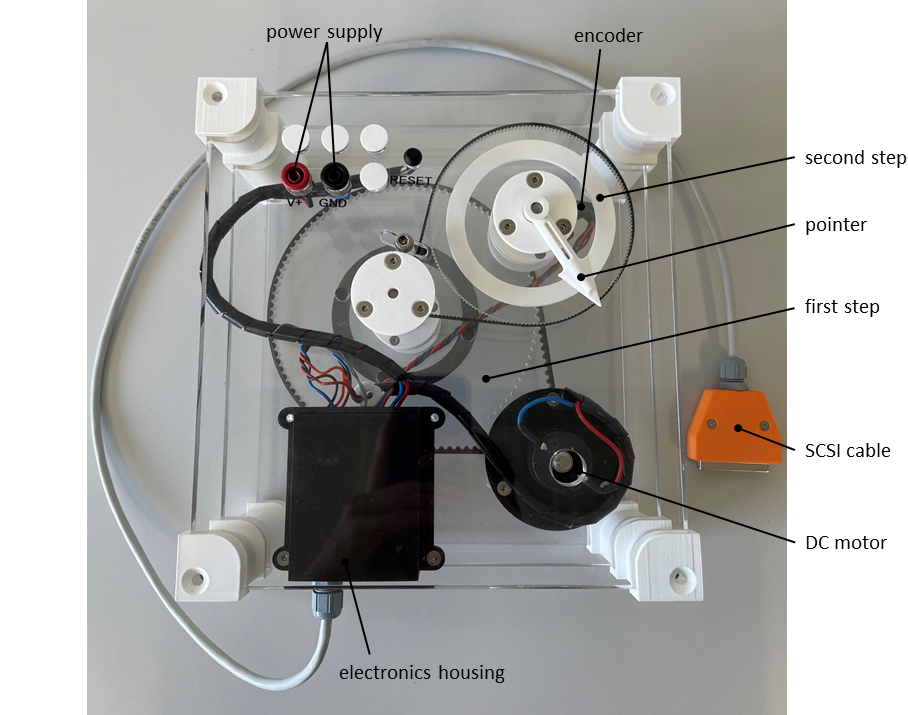
\includegraphics[width=0.75\textwidth]{img/test_bench.png}
  \caption[Test bench with labelled components]{Mechanical belt transmission
    system driven by a DC motor with labelled components\autocite{laboranleitung}}
  \label{fig:testbench}
\end{figure}

\begin{figure}[H]
  \centering
  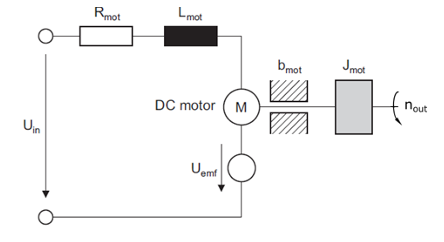
\includegraphics[width=0.6\textwidth]{img/Schematic representation of the electro-mechanical system.png}
  \caption[Schematic representation of the DC motor]{Schematic representation
    of the electro-mechanical system of the DC motor\autocite{laboranleitung}}
  \label{fig:schematic}
\end{figure}

% =====================================================================
\chapter{Preparatory System Identification}\label{app:prep}
% Quelle: Preparation2.m (Ergebnisse der Gruppe), Daten: measurement_data.mat [1]
% data/preparation_step.csv: Rohdaten + Modellkurve aus pt2_model() mit den Ergebnissen
As preparatory work, the step response of an arbitrary mechatronic system is
identified. The measurement data are provided in the file
\texttt{measurement\_\allowbreak data.mat}\autocite{laboranleitung}.
Since the output reacts only after a delay, the PT2 element of
Equation~\eqref{eq:pt2} is extended by a dead time $T_\mathrm{t}$ according to
Equation~\eqref{eq:pt2dead}.
\begin{equation}
  G(s) = \frac{K\,\mathrm{e}^{-T_\mathrm{t} s}}{(\tau_1 s + 1)(\tau_2 s + 1)}
  \label{eq:pt2dead}
\end{equation}
The measured output voltage is normalised to the step amplitude of
\qty{5.24}{\volt}, and the parameters are determined by a least-squares fit with
the MATLAB function \texttt{lsqcurvefit}. The fit yields $K = \num{4.9344}$,
$\tau_1 = \qty{0.0931}{\second}$, $\tau_2 = \qty{0.0253}{\second}$ and
$T_\mathrm{t} = \qty{0.3140}{\second}$. The raw measurement data and the step
response of the identified model are shown in Figure~\ref{fig:prep}.

\begin{figure}[H]
  \centering
  \begin{tikzpicture}
    \begin{axis}[
        width=0.8\textwidth, height=0.42\textwidth,
        xlabel={$t$/\unit{\second}}, ylabel={$u$/\unit{\volt}},
        xmin=0, xmax=2.5, ymin=0, ymax=30,
        grid=major, grid style={gray!30},
        legend style={at={(0.97,0.26)}, anchor=south east}, legend cell align=left,
        /pgf/number format/.cd, use period,
      ]
      \addplot[black, dashdotted, thick] table[x=t, y=u_in, col sep=comma] {data/preparation_step.csv};
      \addlegendentry{input voltage $u_\mathrm{in}$}
      \addplot[gray, thin] table[x=t, y=u_out, col sep=comma] {data/preparation_step.csv};
      \addlegendentry{measured output voltage $u_\mathrm{out}$}
      \addplot[black, dashed, thick] table[x=t, y=u_model, col sep=comma] {data/preparation_step.csv};
      \addlegendentry{identified PT2 model with dead time}
    \end{axis}
  \end{tikzpicture}
  \caption[Preparatory identification of a PT2 element]{Raw measurement data of
    the step response provided in\autocite{laboranleitung} (input dash-dotted,
    output grey) and step response of the identified PT2 model with dead time
    (dashed)}
  \label{fig:prep}
\end{figure}

% =====================================================================
\chapter{Measured Step Responses}\label{app:steps}
% Daten: M1--M8; Kennwerte in Table~\ref{tab:runs}
The measured step responses of all runs in Table~\ref{tab:runs} are shown in
Figures~\ref{fig:run1} to~\ref{fig:run8}.

\begin{figure}[H]
  \begin{floatrow}
    \steprunfig{M1}{1}{195}{22.2}{4.28}
    \steprunfig{M2}{2}{195}{2219.7}{4.28}
  \end{floatrow}
\end{figure}
\begin{figure}[H]
  \begin{floatrow}
    \steprunfig{M3}{3}{1}{22.2}{4.28}
    \steprunfig{M4}{4}{20}{22.2}{4.28}
  \end{floatrow}
\end{figure}
\begin{figure}[H]
  \begin{floatrow}
    \steprunfig{M5}{5}{195}{22.2}{8.00}
    \steprunfig{M6}{6}{195}{22.2}{1.00}
  \end{floatrow}
\end{figure}
\begin{figure}[H]
  \begin{floatrow}
    \steprunfig{M7}{7}{300}{22.2}{4.28}
    \steprunfig{M8}{8}{300}{22.2}{6.00}
  \end{floatrow}
\end{figure}

% =====================================================================
\chapter{Disturbance and Sinusoidal Reference}\label{app:data}
% Daten: disturbance, sine ... sine5 (matlab.mat); Sinus-Parameter aus RunPositionController1.slx
% Beobachtungen aus Controll_eng_pid_tuning.xlsx
Figure~\ref{fig:disturbance} shows the reaction to a disturbance applied manually to the
pointer with the controller gains of run~1. For the tracking of a sinusoidal
reference with an amplitude of \ang{10} and an angular frequency of
\qty{5}{\radian\per\second}, $K_\mathrm{P}$ is varied while $K_\mathrm{I}$ and
$K_\mathrm{D}$ are kept constant. The observations are listed in
Table~\ref{tab:sine}; the tracking is shown
in Figure~\ref{fig:sine-track}, and the control error and control value for each
gain in Figures~\ref{fig:sine195} to~\ref{fig:sine1200}.

\begin{figure}[H]
  \centering
  \begin{tikzpicture}
    \begin{axis}[
        width=0.8\textwidth, height=0.36\textwidth,
        xlabel={$t$/\unit{\second}}, ylabel={$\theta$/\unit{\degree}},
        xmin=1, xmax=10, ymin=43, ymax=48,
        grid=major, grid style={gray!30},
        legend pos=north east, legend cell align=left,
        /pgf/number format/.cd, use period,
      ]
      \addplot[black, thick] table[x=t, y=theta, col sep=comma] {data/disturbance.csv};
      \addlegendentry{measured}
      \addplot[black, dotted, thick] table[x=t, y=ref, col sep=comma] {data/disturbance.csv};
      \addlegendentry{reference}
    \end{axis}
  \end{tikzpicture}
  \caption[Reaction to a disturbance]{Measured angular position after the
    reference step of \ang{45} with a disturbance applied manually to the pointer
    (controller gains of run~1, section from \qtyrange{1}{10}{\second})}
  \label{fig:disturbance}
\end{figure}

\begin{table}[H]
  \centering
  \caption[Tracking of a sinusoidal reference]{Proportional gains and
    observations for the tracking of a sinusoidal reference (amplitude \ang{10},
    angular frequency \qty{5}{\radian\per\second}) with
    $K_\mathrm{I} = \qty{22.2}{\volt\per\radian\per\second}$ and
    $K_\mathrm{D} = \qty{4.28}{\volt\second\per\radian}$}
  \label{tab:sine}
  \begin{tabular}{S[table-format=4.0] l}
    \toprule
    {$K_\mathrm{P}$/(\unit{\volt\per\radian})} & Observation \\
    \midrule
     195 & slightly slow \\
     300 & control error halved \\
     600 & control error further reduced \\
     800 & control value too noisy \\
    1200 & control value strongly noisy \\
    \bottomrule
  \end{tabular}
\end{table}

\begin{figure}[H]
  \centering
  \begin{tikzpicture}
    \begin{axis}[
        width=0.8\textwidth, height=0.36\textwidth,
        xlabel={$t$/\unit{\second}}, ylabel={$\theta$/\unit{\degree}},
        xmin=0, xmax=10, ymin=-15, ymax=20,
        grid=major, grid style={gray!30},
        legend pos=north east, legend columns=2, legend cell align=left,
        /pgf/number format/.cd, use period,
      ]
      \addplot[black, thick] table[x=t, y=theta, col sep=comma] {data/sine.csv};
      \addlegendentry{measured}
      \addplot[black, dotted, thick] table[x=t, y=ref, col sep=comma] {data/sine.csv};
      \addlegendentry{reference}
    \end{axis}
  \end{tikzpicture}
  \caption[Tracking of a sinusoidal reference]{Measured angular position and
    sinusoidal reference for $K_\mathrm{P} = \qty{195}{\volt\per\radian}$}
  \label{fig:sine-track}
\end{figure}

\begin{figure}[H]
  \begin{floatrow}
    \sinerunfig{sine}{195}{fig:sine195}
    \sinerunfig{sine2}{300}{fig:sine300}
  \end{floatrow}
\end{figure}
\begin{figure}[H]
  \begin{floatrow}
    \sinerunfig{sine3}{600}{fig:sine600}
    \sinerunfig{sine5}{800}{fig:sine800}
  \end{floatrow}
\end{figure}
\begin{figure}[H]
  \begin{floatrow}
    \sinerunfig{sine4}{1200}{fig:sine1200}
  \end{floatrow}
\end{figure}


\end{document}